% 2009 年重庆卷理科第 20 题：椭圆 x^2+y^2/4=1、单位圆与点 A、B、M、N、Q。
% 来源 PDF：普通高考/2009/2009重庆理.pdf，SHA-256 6a815fa472e380a3f1143e8cdd93712e142309acb7a95176783499406a8e15f1。
% 原页：第 2 页（A3 三栏）第 2 栏中部，书页码 504。
% 重绘依据：按更正后的椭圆 x^2+y^2/4=1 绘制；取 M(0.8,1.2)、N(0.8,0)、Q(1.6,1.2)，
%   B 取单位圆上满足 QA⊥BA 的点 (-0.6,0.8)，仅作示意。
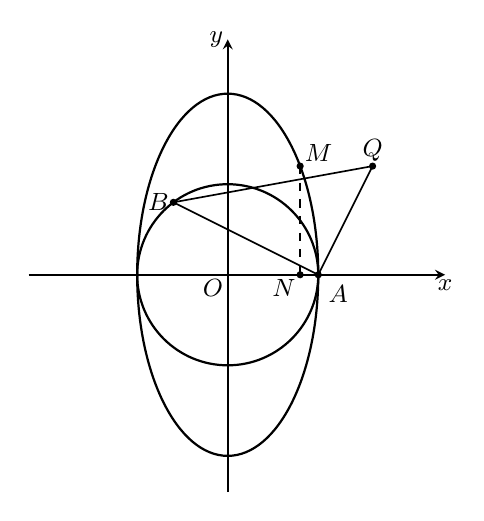
\begin{tikzpicture}[semithick, x=1.15cm, y=1.15cm, every node/.style={inner sep=1.4pt, font=\small}]
  % 坐标轴
  \draw[-stealth] (-2.2,0) -- (2.4,0) node[below] {$x$};
  \draw[-stealth] (0,-2.4) -- (0,2.6) node[left] {$y$};
  \node[below left] at (0,0) {$O$};

  % 椭圆
  \draw[thick] (0,0) ellipse (1 and 2);
  % 单位圆
  \draw[thick] (0,0) circle (1);

  % 点
  \coordinate (A) at (1.0,0.0);
  \coordinate (M) at (0.8,1.2);
  \coordinate (N) at (0.8,0.0);
  \coordinate (Q) at (1.6,1.2);
  \coordinate (B) at (-0.6,0.8);
  \fill (A) circle (1.3pt);
  \fill (M) circle (1.3pt);
  \fill (N) circle (1.3pt);
  \fill (Q) circle (1.3pt);
  \fill (B) circle (1.3pt);

  % 辅助线
  \draw[dashed] (M) -- (N);
  \draw (Q) -- (B);
  \draw (Q) -- (A);
  \draw (A) -- (B);

  % 标注
  \node[below right=2pt] at (A) {$A$};
  \node[above right] at (M) {$M$};
  \node[below left] at (N) {$N$};
  \node[above] at (Q) {$Q$};
  \node[left] at (B) {$B$};
\end{tikzpicture}
